\begin{titlepage}
  \begin{center}
    \large
 
 	МОСКОВСКИЙ ГОСУДАРСТВЕННЫЙ УНИВЕРСИТЕТ ИМЕНИ М. В. ЛОМОНОСОВА

    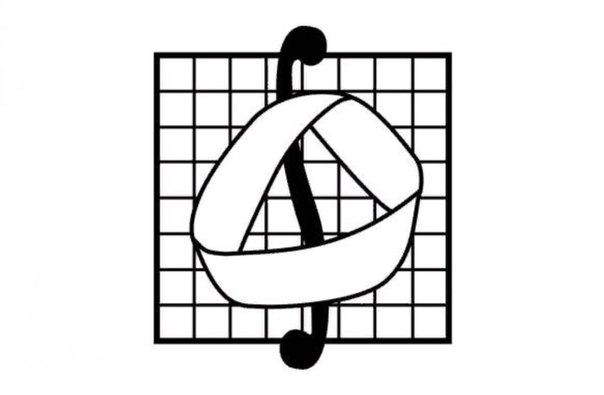
\includegraphics[scale=0.6]{mm.jpg} 
     
    Механико-математический факультет
    \vspace{0.25cm}

    Кафедра Вычислительной Математики
    \vspace{0.25cm}
 
    \textsc{Курсовая работа}\\[5mm]
     
    {\LARGE Восстановления отрезка по проекциям на плоскостях}
    \bigskip

    Конов Марк Андреевич
    \vspace{0.25cm}
     
    3 курс, группа 332
\end{center}
\vfill
 
\newlength{\ML}
\settowidth{\ML}{«\underline{\hspace{0.7cm}}» \underline{\hspace{2cm}}}
\hfill\begin{minipage}{0.5\textwidth}
  \begin{flushright}
     Научный руководитель\\
    к.ф.-м.н. \\
    Валединский Владимир Дмитриевич\\
    «\underline{\hspace{0.7cm}}» \underline{\hspace{2cm}} 2021 г.
  \end{flushright}
\end{minipage}%
\vfill
\bigskip
 
\begin{center}
  Москва, 2021 г.
\end{center}
\end{titlepage}
\newpage